\section{Erstellung eines Modells zur Bodenatmung}
\label{sec-model}

\subsection{Korrelationsanalyse}

\begin{figure}
	\centering
	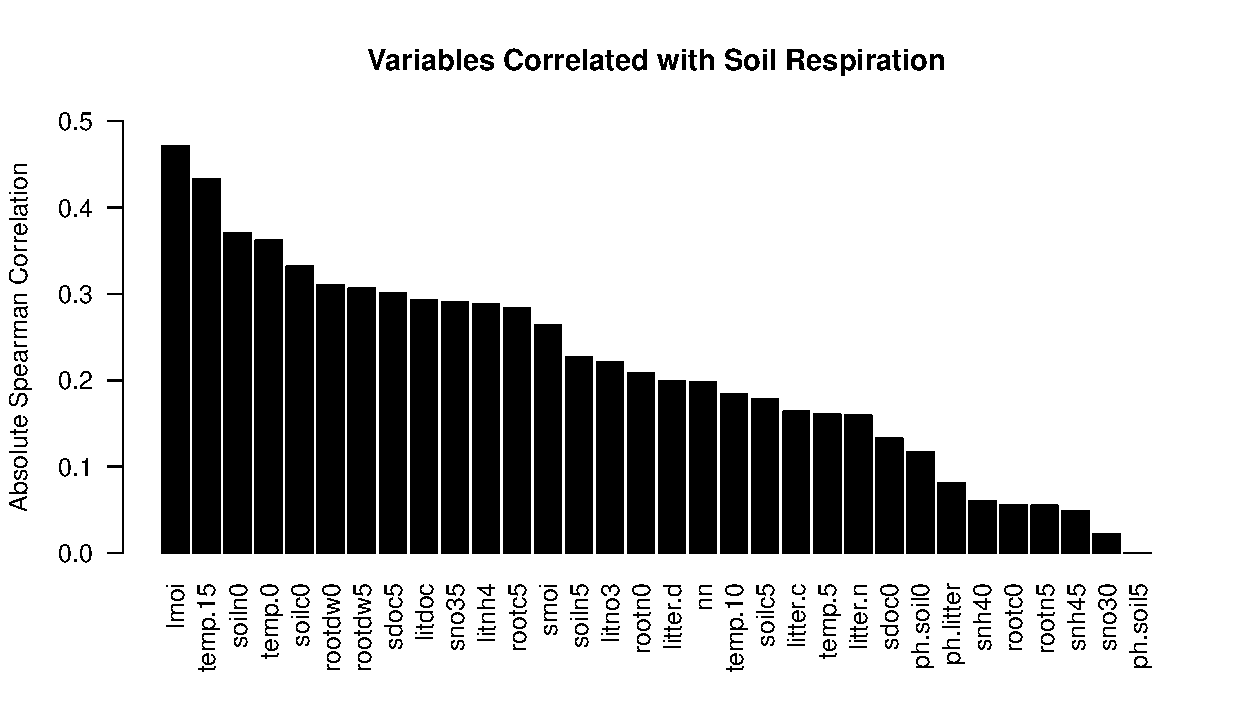
\includegraphics[width=\textwidth]{fig/model/spearsman-cor.pdf}
	\caption{\bf{Spearsman-Korrelation} der Einflussgrößen mit der Bodenatmung.}
\end{figure}

\subsection{Transformationen}
$exp(Tmp)$ anstatt $Tmp$?

\subsection{Variabelnselektion}

\subsection{Ergebnis}
Qualität des gewählten Modells

\subsection{Umsetzung mit R}

\begin{lstlisting}
## corelation
#correlation from soil.res with all others
hainich.r <- abs(cor(hainich, method = "pearson"))["soil.res",-1]
hainich.r.ordered <- hainich.r[order(hainich.r, decreasing = T)]
barplot(hainich.r.ordered, las = 2, ylim = c(0,0.5), col = "black", 
ylab = "Absolute Pearson Correlation", main = "Variables Correlated with Soil Respiration")

## scatter plot
pairs(~ rootdw0 + smoi + nn,
data = hainich, main = "Scatterplot Matrix")
\end{lstlisting}